\section{The Armory}

\vspace{5mm}

\subsection*{C.E.D.R.I.C} 

\begin{center}
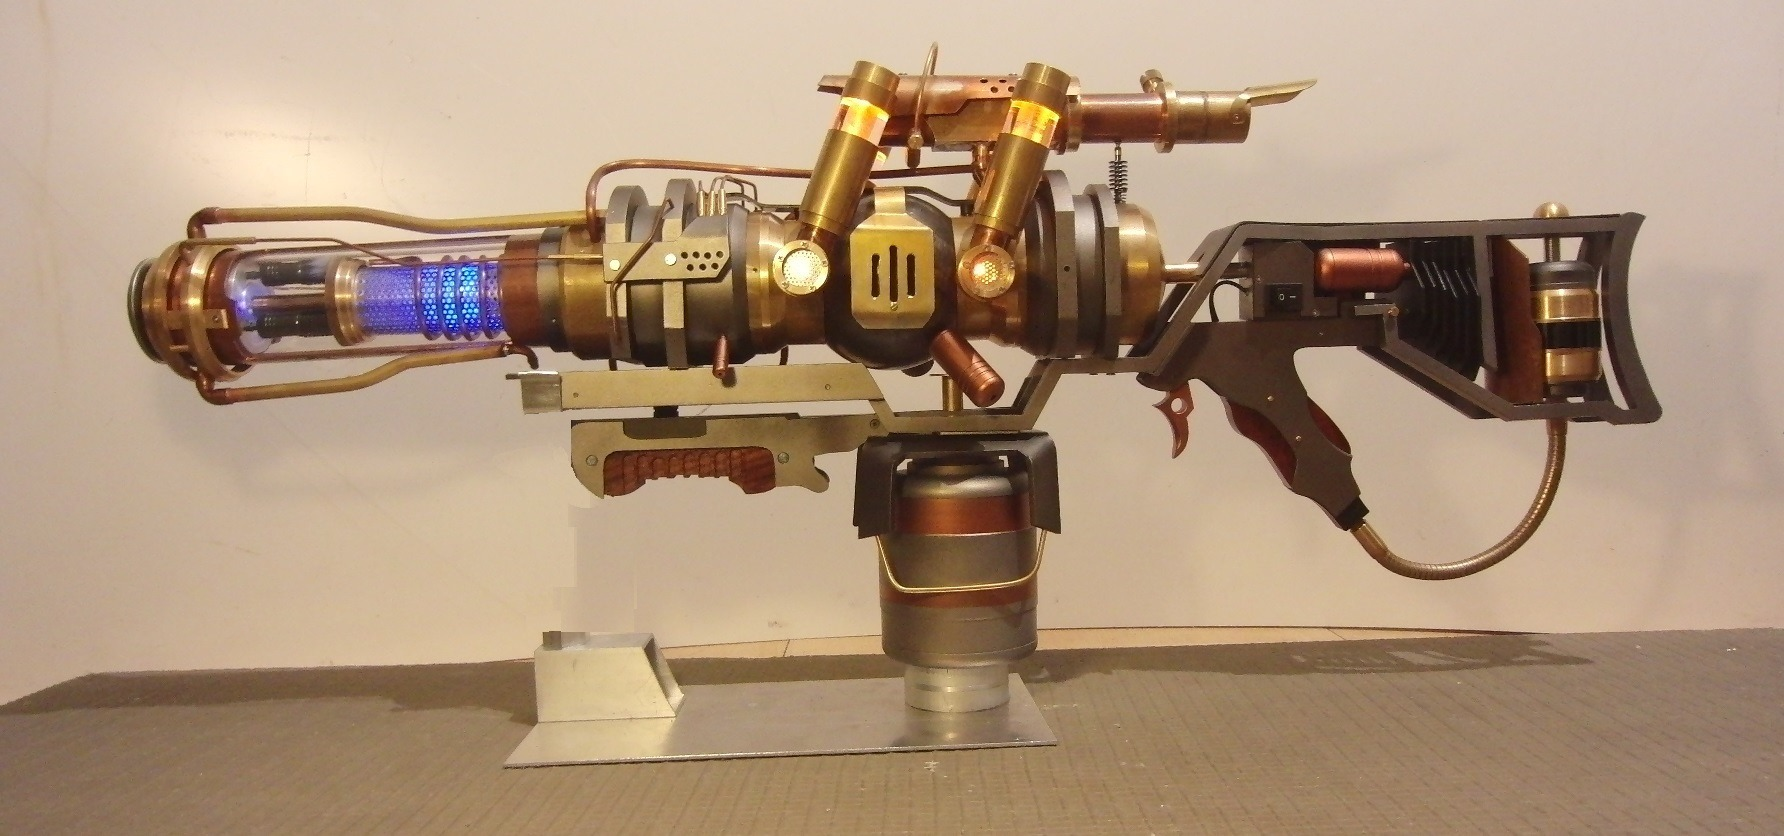
\includegraphics[width=80mm]{./content/img/cedric.jpg}
\begin{figure}[h]
\end{figure}
\end{center}

\noindent 

'Collaborative Experimental Destruction and Rapid Immolation Contraption'.  A sentient weapon that grants several tactially advantageuous improvements to perception and can actively retarget low damage shots.  The weapon also has the ability to imrpvoe the speed of it's user greatly. 

\smallskip



\subsection*{Godbringer} 

\begin{center}
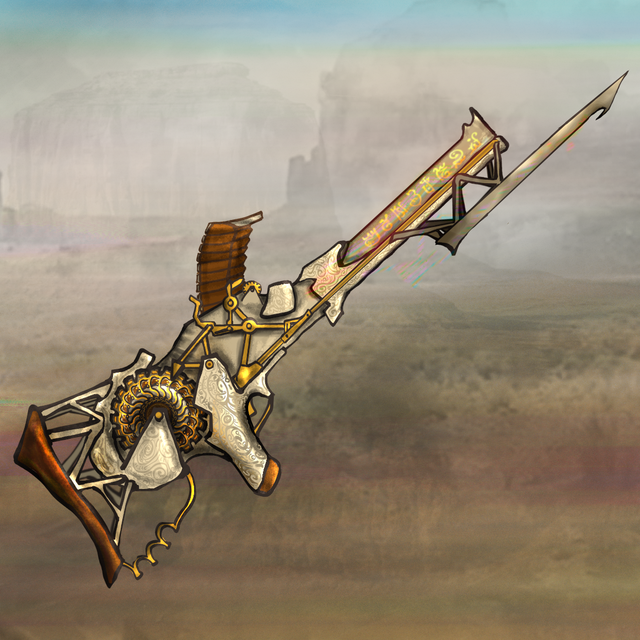
\includegraphics[width=80mm]{./content/img/godbringer.png}
\begin{figure}[h]
\end{figure}
\end{center}

\noindent 

Text

\smallskip



\subsection*{Myron's Shield} 

\begin{center}
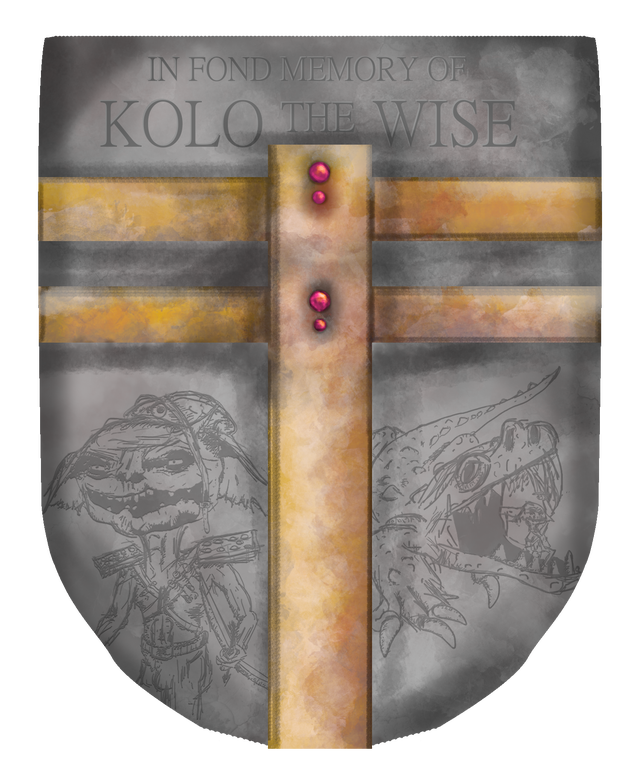
\includegraphics[width=80mm]{./content/img/koloShield.png}
\begin{figure}[h]
\end{figure}
\end{center}

\noindent 

Text

\smallskip



\subsection*{Shocking Gloves} 

\begin{center}
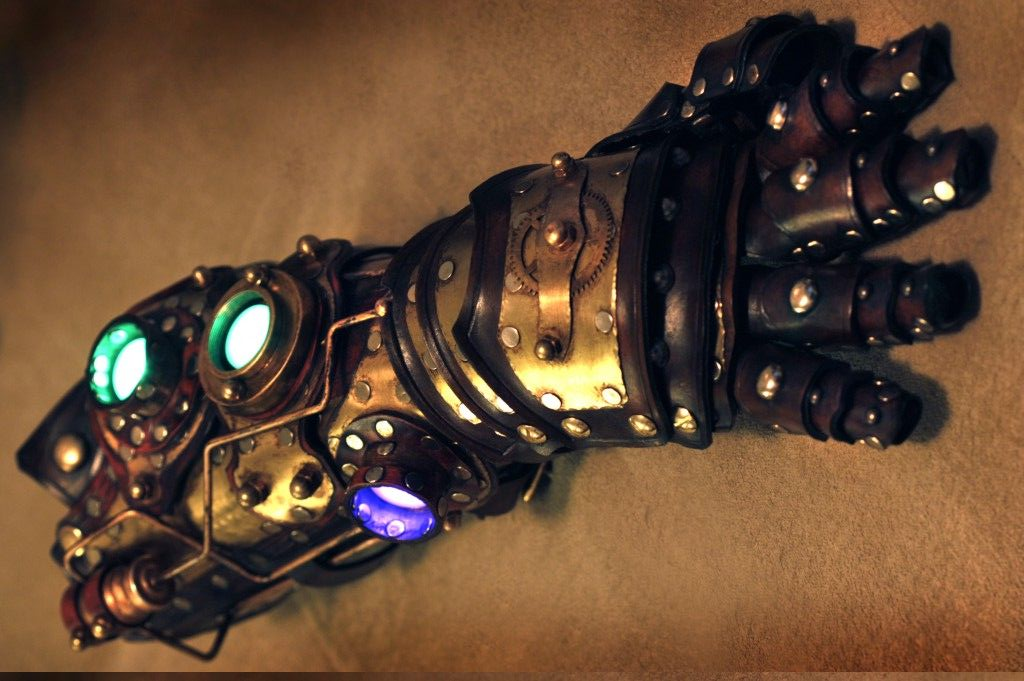
\includegraphics[width=80mm]{./content/img/gloves.jpg}
\begin{figure}[h]
\end{figure}
\end{center}

\noindent 

Crafted from the "Lord of Lightning" - an electric beast. A pair of gloves attached to a small device on the hip that give their wielders the ability to deliver shocks.

Can deliver a powerful electric shock, recharging after the wielder has moved 100 yards. Secondarily can be used to stabilise a dying creature.

\smallskip

\subsection*{Black Sabbath} 

\begin{center}
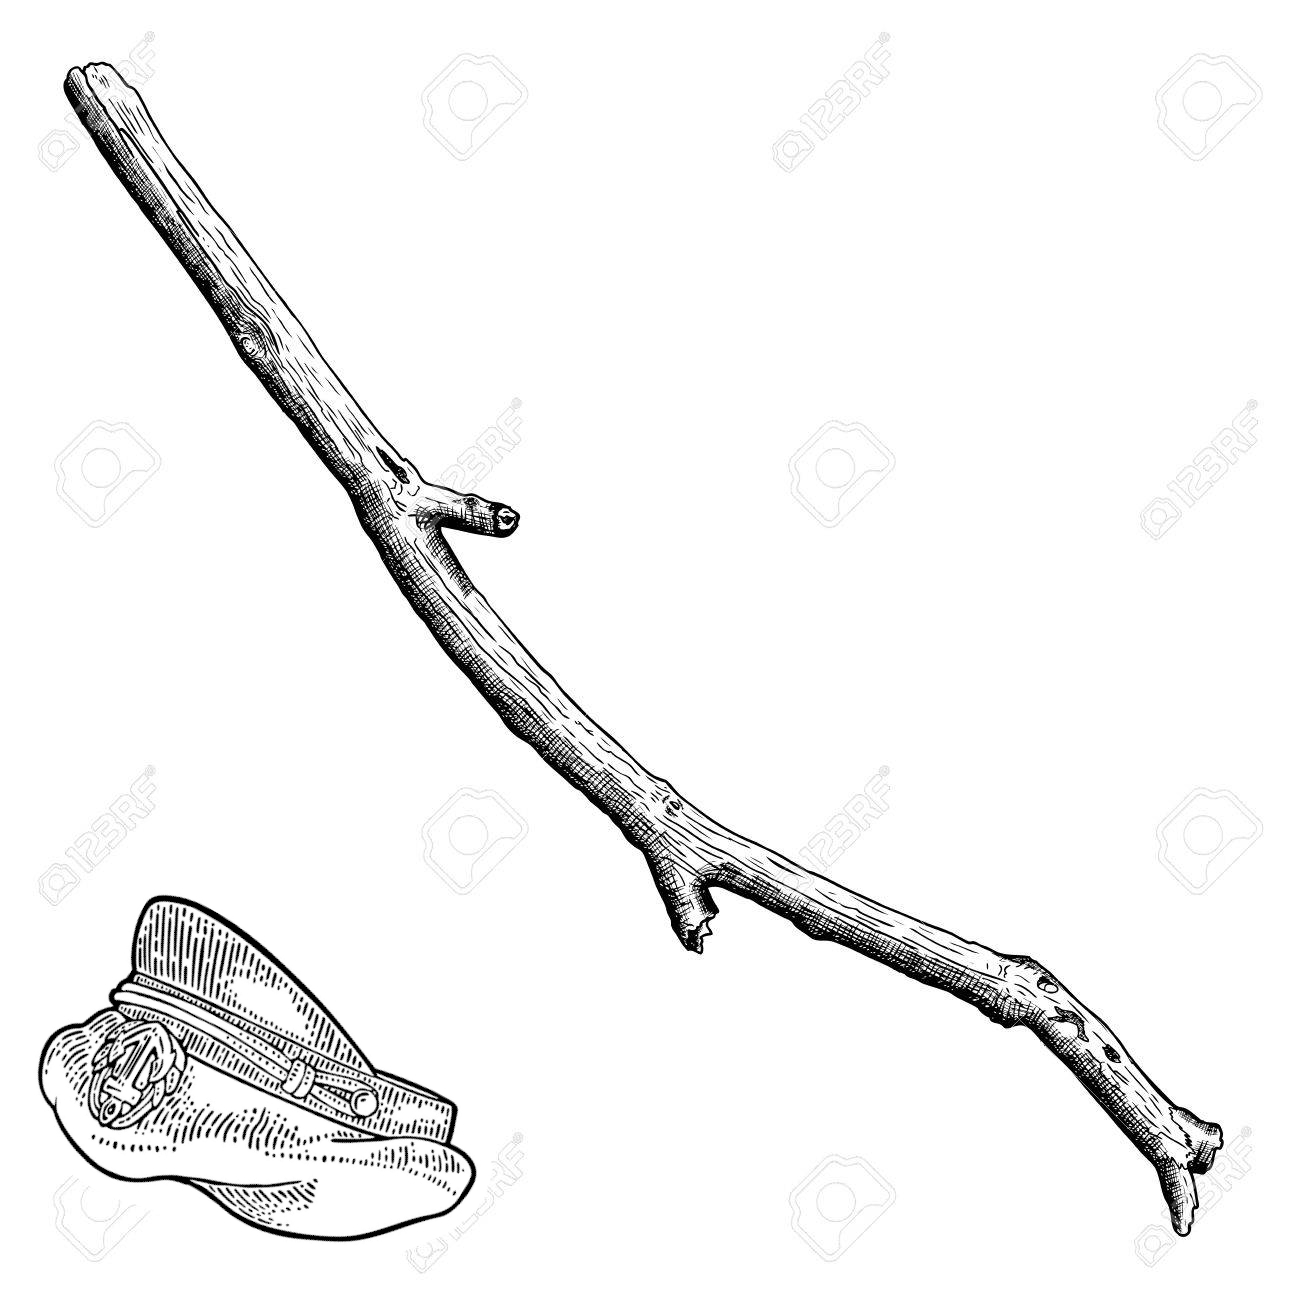
\includegraphics[width=80mm]{./content/img/xxx.png}
\begin{figure}[h]
\end{figure}
\end{center}

\noindent 

Former Two Handed pronged shadow-blade forged from shadow sorcery and the Stone of Unthala.

Can surge shadows to inflict heavy damage to a target - sadly unstable and potentially poisons the wielder

\smallskip

\subsection*{Iron Maiden} 

\begin{center}
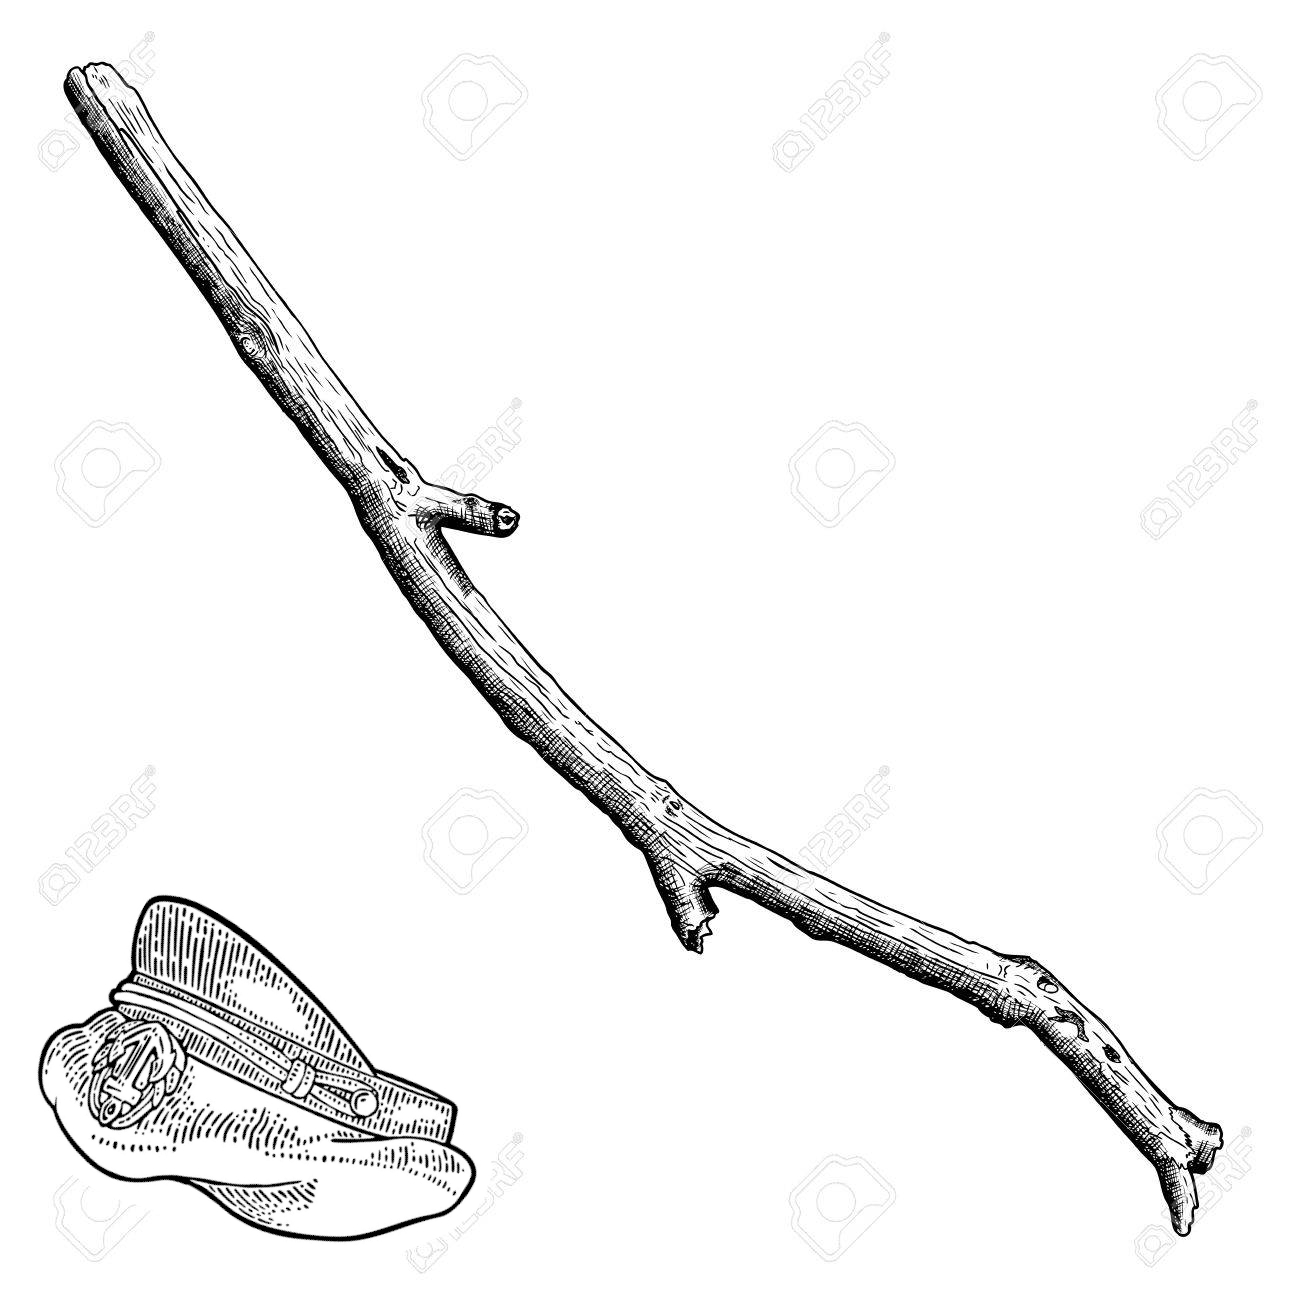
\includegraphics[width=80mm]{./content/img/xxx.png}
\begin{figure}[h]
\end{figure}
\end{center}

\noindent 

One handed katana that originally felled Otario, was reforged from Black Sabbath.

Slightly better than before being magical, may have hidden talents. Nonmagical (less magical) since Pilch died.

\smallskip

\subsection*{Bow of the Bastard} 

\begin{center}
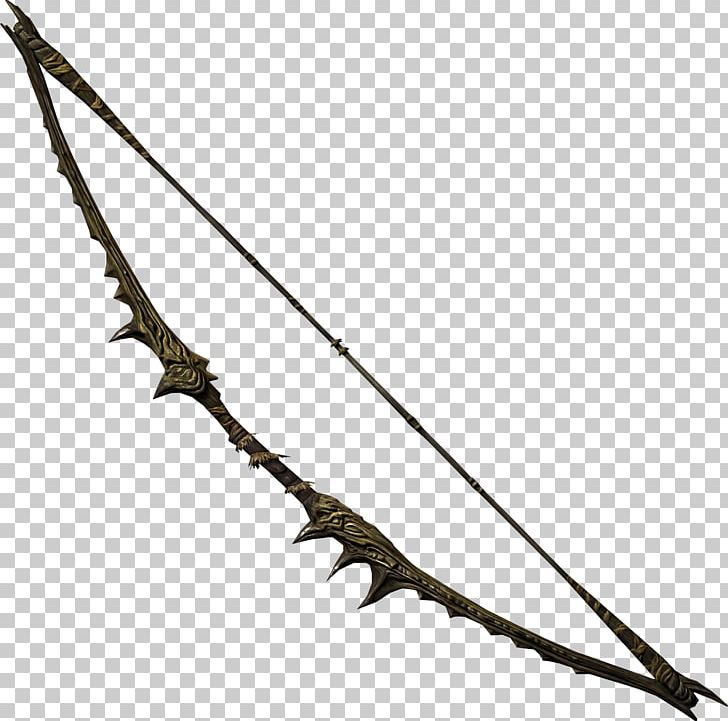
\includegraphics[width=80mm]{./content/img/bastardBow.jpg}
\begin{figure}[h]
\end{figure}
\end{center}

\noindent 

An highly accurate short-bow, believed to have belonged to (and potentially been crafted by) a halfling thief centuries ago - nicknamed "The Little Bastard". It has secondary properties related to hurting a target for more damage.

In addition to being a magical shortbow, if the wielder manages to hit a surprised target that target takes additional damage (3d6) - but the wielder of the bow will be less charismatic (disadvantage on charisma rolls) until they next have a short rest, as everyone views them as a bastard.

\smallskip

\subsection*{Hammer of the Gods} 

\begin{center}
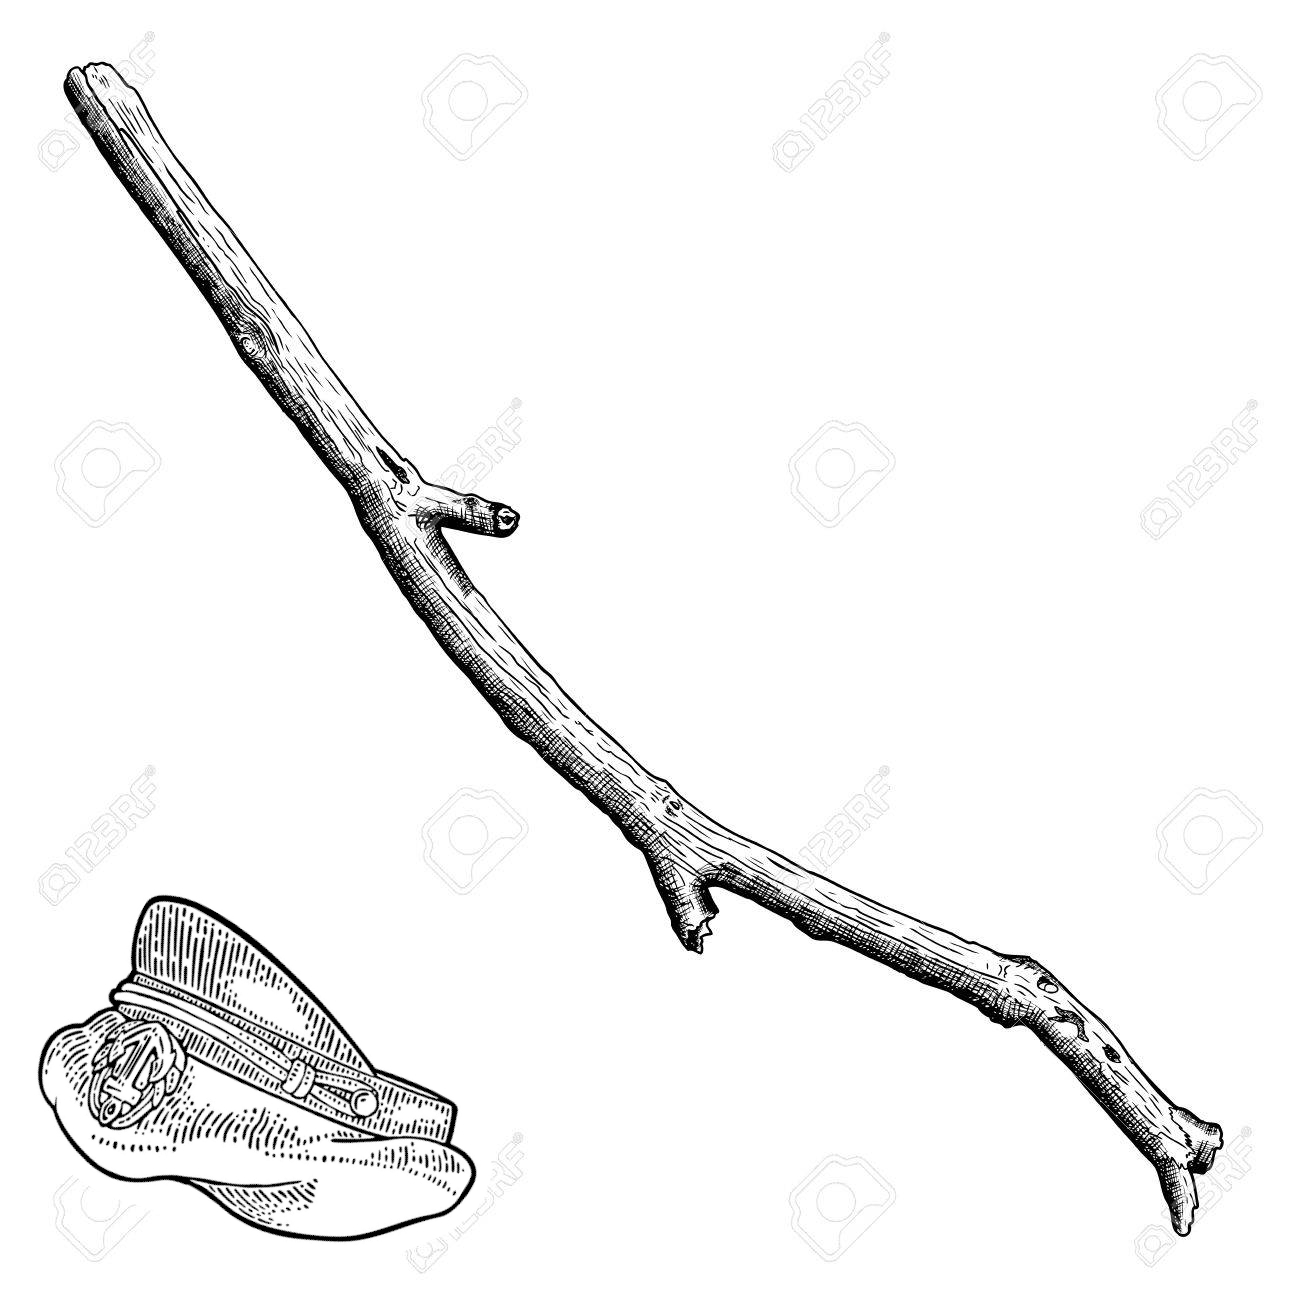
\includegraphics[width=80mm]{./content/img/xxx.png}
\begin{figure}[h]
\end{figure}
\end{center}

\noindent 

Used in ancient Crusades by the Zealot Arbiter Elron, when he travelled east to Masuda, said to defeat an Inthun infused Varg in a single blow (so may be made of starmetal).

\begin{DndComment}{Extract from ''The Lands of the Godless"}
Excursions to the East have met with mixed success over the years. There has always been a strong desire amongst the faithful to bring the light of the gods to the heathen lands. The question of how best to approach this has led to many missteps and failings. I write this treatise in the hopes that future generations will learn from the mistakes of the past in future endeavours.

Firstly, knowledge of the culture of the lands is essential to the success of any conversion. The first voyagers failed when they approached the peoples of Masuda in the same way they approached those of Nanduan. While they may look similar, the cultures vary in insurmountable ways. The people of Nanduan have been resistant to all forms of preaching, while a foothold has eventually been made in Masuda albeit in small ways.

More success has been found with peaceful approaches to the eastern lands. Much can be learned from the failed crusade of the zealot arbiter Elron. He bore the Hammer of the Gods, a weapon so powerful it struck down even the Inthun-infused terror of Hunthar Varg and ended the third Varghold incursion in a single fiery blow. With such power behind him and an army of arbiters, Elron sailed East to deliver ‘holy justice’ to the unbelievers.

The Masudan response to such an invasion was, by all accounts, as brutal as it was swift. Few survivors returned, and those who did told tale of a dawn assault by incredibly skilled swordsmen with lightning fast blades. As they tried to react it soon became clear that Elron and all the commanding officers had been slain during the night, their throats slit by assassins that slipped past even the most perceptive guards.

The Hammer of the Gods itself was lost during that fateful voyage, a lesson in humility to all our followers. Let it be known that when we approach with brutality the Gods will show us no clemency. We must spread our message with the light and fairness in which it was intended.
\end{DndComment}

\smallskip







\clearpage